\documentclass[12pt]{article}

\newcommand{\bi}{\begin{itemize}}
\newcommand{\ei}{\end{itemize}}
\newcommand{\be}{\begin{enumerate}}
\newcommand{\ee}{\end{enumerate}}
\newcommand{\code}[1]{\texttt{#1}}

\usepackage{enumitem}
\usepackage[margin=1in]{geometry}
\usepackage{graphicx}

\usepackage{hyperref}
\hypersetup{
    colorlinks=true,
    linkcolor=black,
    filecolor=magenta,      
    urlcolor=cyan,
}
\urlstyle{same}

\graphicspath{ {./images/} }

\setlistdepth{6}
\renewlist{itemize}{itemize}{6}
\setlist[itemize]{label=$\cdot$}

\begin{document}

\begin{center}
    \vspace*{\fill}
  {\large \textbf{``Cash Me A Taxi"}}\\[2mm]
  {\large \textbf{Design Specifications Document}}\\[2mm]
  {\large \textbf{SFRWENG 2XB3 - L03 Group 7}}\\[8mm]
  {\large Albert Zhou, zhouj103}\\[2mm]
  {\large Areeba Aziz, aziza11}\\[2mm]
  {\large David Bednar, bednad1}\\[2mm]
  {\large Dylan Smith, smithd35}\\[2mm]
  {\large Himanshu Aggarwal, aggarwah}\\[6mm]
  {\large Department of Computing and Software, McMaster University}\\[6mm]
  {\large \today}
  \vspace*{\fill}
\end{center}

\newpage

\section*{Revisions}

\begin{center}
\begin{tabular}{|c|c|c|}
\cline{1-3}
\textbf{Member} & \textbf{Student Number} & \textbf{Role}\\
\cline{1-3}
Albert Zhou & 400196651 & GUI\\
\cline{1-3}
Areeba Aziz & 400070863 & Data Structure Designer\\
\cline{1-3}
David Bednar & 400177661 & Algorithms\\
\cline{1-3}
Dylan Smith & 001314410 & Client\\
\cline{1-3}
Himanshu Aggarwal & 400200223 & Testing\\

\cline{1-3}
\end{tabular}
\end{center}

\noindent \emph{By virtue of submitting this document we electronically sign and date that the work being submitted by all the individuals in the group is their exclusive work as a group and we consent to make available the application developed through SE-2XB3 project, the reports, presentations, and assignments (not including my name and student number) for future teaching purposes}

\newpage

\section*{Contributions}

\begin{tabular}{|p{4cm}|p{5.5cm}|p{7cm}|}
\hline
\textbf{Name} & \textbf{Role} & \textbf{Contributions}\\
\hline
Albert Zhou & GUI & GUI \newline Report Structure \newline GraphFinder \newline Diagrams \newline Requirements traceback \\
\hline
Areeba Aziz & Data Structure Designer & GUI and Cmd-line Controllers \newline GraphSearch \newline File Writer Helper \newline GraphFileController \newline Report finalization\\
\hline
David Bednar & Algorithms & Sorters \newline Models (Graph, Node, Edge) \\
\hline
Dylan Smith & Client & Parser \\
\hline
Himanshu Aggarwal & Testing & Test classes \newline Trip ADT\\
\hline
\end{tabular}

\newpage

\section*{Executive Summary}
This project intends to provide a solution for the problem of taxi drivers in New York City
struggling financially as modern ride-sharing apps like Uber currently dominate the market. The solution is to calculate the most optimal routes between NYC zones that earn drivers the most profit, based on 10 years’ worth of taxi trips datasets provided by the City of New York. The datasets contain taxi trip data such as the distance travelled per trip, the amount of fare made, the tips earned, and the start/end location and times. \\ \\
Our program first parses the intensive data that contains the taxi trip records and builds a directed graph with nodes representing a NYC taxi zone. The user then can select from various functions to run on the graph, such as search for the most optimal path between two given zones, or sort the edges (routes) by the given field (fare, tip, distance, etc). This project implements graph traversal, sorting and searching algorithms that were taught throughout the year. 

\newpage

\tableofcontents

\newpage

\section{Deployment Guide}

\subsection{Installation and Setup}
\be
	\item Download the Eclipse project and open it on Eclipse. 
	\item To run the GUI Application, open the \code{GUI.java} file and then click on the Run button on Eclipse. 
	\item To run the Command-line Application, navigate to the \code{Main.java} file. From the top menu on Eclipse, go to Run $\rightarrow$ Run configurations $\rightarrow$ Arguments. Enter your Program arguments which must match the format specified in the \hyperref[sec:cmdlineinterface]{\textcolor{blue}{command-line interface specifications}}. 
	\item To run automated tests, navigate to the \code{AllTests.java} file, and then click the Run button on Eclipse.
\ee

\subsection{Prerequisite Knowledge}
In this section we will outline some basic information that you'll need to know in order to use our application.
\bi
	\item This application uses datasets on taxi trip records provided by the City of New York. There are 10 years' worth of extensive data available to the public here:\\ \url{https://www1.nyc.gov/site/tlc/about/tlc-trip-record-data.page}. 
	\item By default, there is 1 dataset that exists within the project, which is the 2019 Yellow Taxi Trip Records. This is the dataset that will be used by default. If you wish to use another dataset from the same website, you may download it and then enter that dataset's file location into the application to use that instead.
	\item A ``zone" is a NYC taxi zone. Each zone has a unique integer zone ID that ranges from 1 to 263. More information about these zones can be found on the end of this webpage: \url{https://www1.nyc.gov/site/tlc/about/tlc-trip-record-data.page}
	\item In our application, we build the graph while parsing the input dataset. The graph contains nodes that represent a NYC zone, and directed edges that represent the aggregate data of trips made between the source zone and the destination zone. Since the input dataset is very large, we save the graph that is constructed onto a csv file for future use. So, if you've run the application once and the graph has been constructed, and then later you want to re-run the application but use the same input dataset as before, instead of re-building the entire graph, you can simply specify the filepath of the graph data file that was generated at the previous application run. This could save a lot of time if you want to aggregate all 10 years' worth of data to run multiple functions on the application. 
\ei

\subsection{GUI Application}
In this section we will provide a complete walk through of the Cash Me A Taxi GUI application. 

\be
	\item {When the app is launched you will be greeted with the following screen.}

    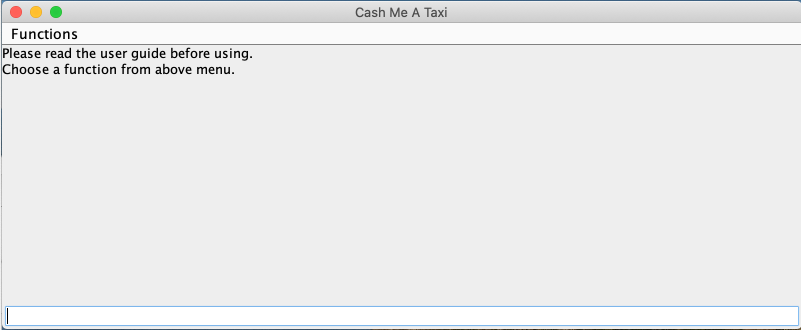
\includegraphics[scale = 1]{Images/StartUpScreen.png} 
    
    \item {To begin using the app, click on ``Functions". A drop-down menu of function options will appear.}
    
    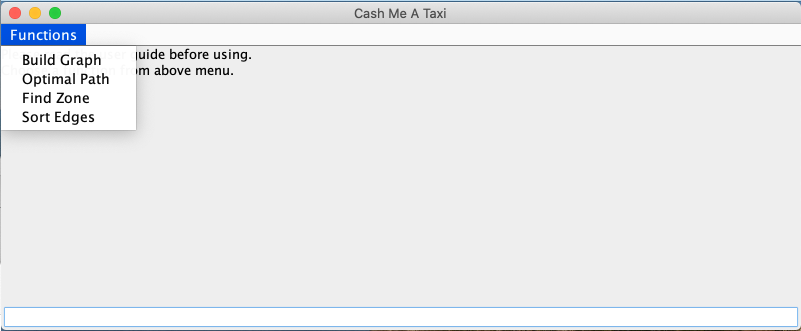
\includegraphics[scale = 1]{Images/FunctionsDropdown.png} 
    
    \item {Select the function you would like to use.}
    \bi
    	\item \textbf{Optimal Path:} Compute the most optimal path from a given start zone and end zone.
    	\item \textbf{Find Zone:} Given a zone ID, find the zone in the list of all zones and get its outgoing edges.
    	\item \textbf{Sort Edges:} Sort all the edges in the graph by a field such as average fare, average tips, etc.
    	\item \textbf{Build Graph:} Only build the graph and save its data onto a file. 
    	\item Note that all functions will build the graph first and then compute the function specified. If you wish to change the data set you must restart the app.
    \ei
\ee

\subsubsection{Build Graph}\label{BuildGraph}
\be
    \item{When ``Build graph" is chosen you will be given the following options.}

    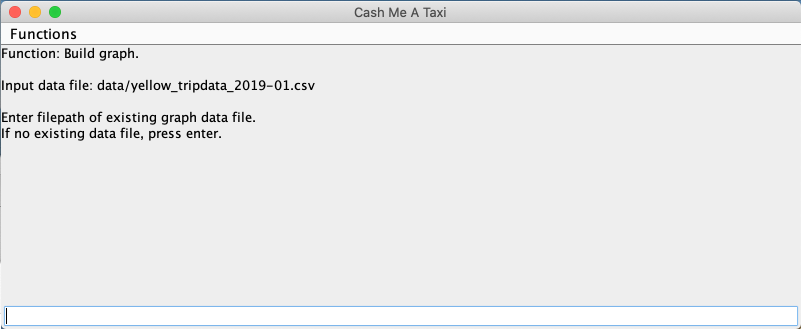
\includegraphics[scale = 1]{Images/BuildGraph.png}
    
    \item {If you have already run the app, and have created a graph data file, you may enter the location of the file. If not, hit enter in the input textbox in the bottom of the screen to skip this step.}
    \item {If you had not specified an existing graph data file, you will now be prompted to enter the file path of the input dataset you would like to use. If you want to use the default input dataset that is included with the application, simply hit enter to skip this step.}

    \item{When the input file has been chosen, the app builds a graph and stores the edges in the file specified. Note this can take around 20 seconds.}
    
    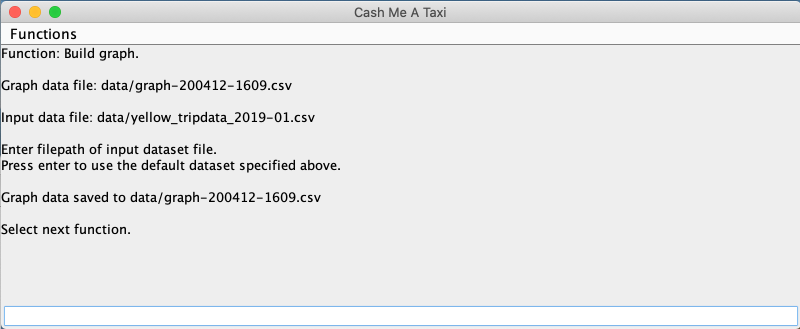
\includegraphics[scale = 1]{Images/BuildGraphOutput.png}
    
    \item{You are now able to choose another function from the ``Functions" menu on the top menu bar.}
\ee

\subsubsection{Optimal Path}
\be
    \item{When ``Optimal Path" is selected, you will be given the following options. (Assuming you have already run the "Build Graph" function. If you have not, you will be prompted to input the file path. Return to \ref{BuildGraph} and repeat steps 2 and 3, before proceeding).}
    
    \item{You are prompted to enter a start and end zone ID, separated by a space. It is assumed that the user will be familiar with the zone IDs of the city. Zones range from 1-263 and can be found at \url{https://www1.nyc.gov/site/tlc/about/tlc-trip-record-data.page}, under Taxi Zone Lookup Table.}
    
    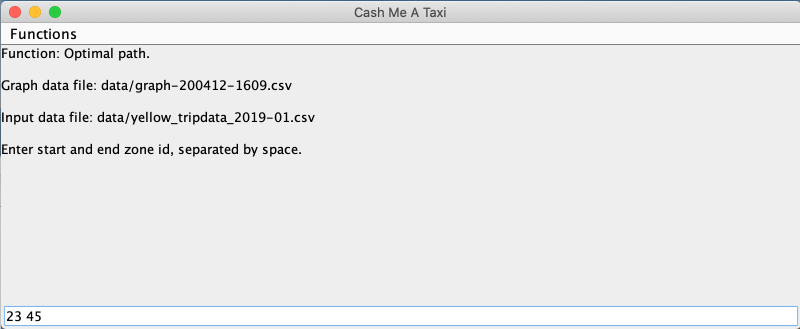
\includegraphics[scale = 1]{Images/OptimalPathData.png}
    
    \item{Once the zone IDs are entered, the app calculates the optimal route and stores it in the file specified. .}
    
    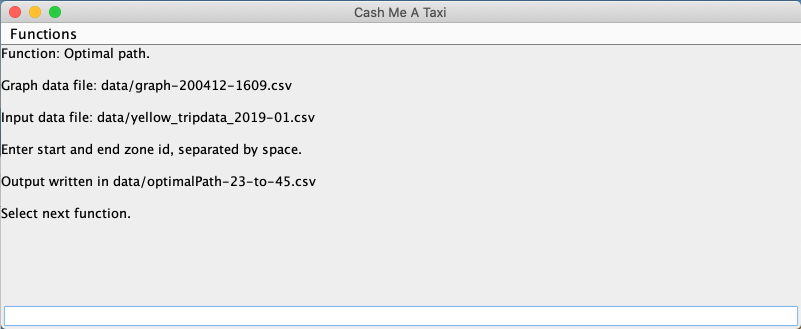
\includegraphics[scale = 1]{Images/OptimalPathOutput.png}
    
    \item{You are now able to choose another function from the ``Functions" menu on the top menu bar.}
\ee

\subsubsection{Find Zone}
\be
    \item{When ``Find Zone" is chosen you will be given the following options. (Assuming you have already run the "Build Graph" function. If you have not, you will be prompted to input the file path. Return to \ref{BuildGraph} and repeat steps 2 and 3, before proceeding).}
       
    \item{You are prompted to enter the zone ID you are looking for. It is assumed the user will be familiar with the zone IDs of the city. Zones range from 1-263 and can be found at \url{https://www1.nyc.gov/site/tlc/about/tlc-trip-record-data.page}, under Taxi Zone Lookup Table.}
     
    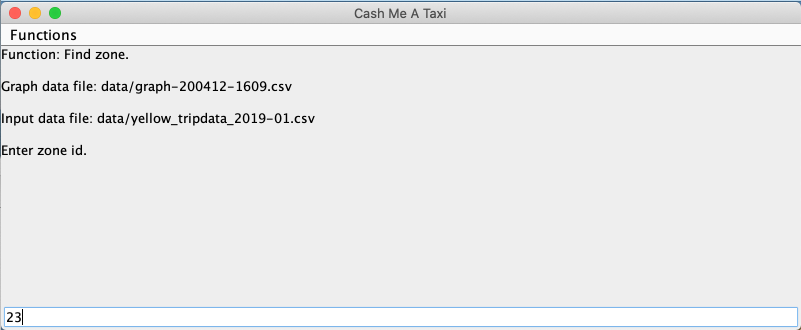
\includegraphics[scale = 1]{Images/FindZoneData.png}
    
    \item{Once the zone ID has been entered, the app searches for the data stored in the node and writes the results to the specified file. }
    
    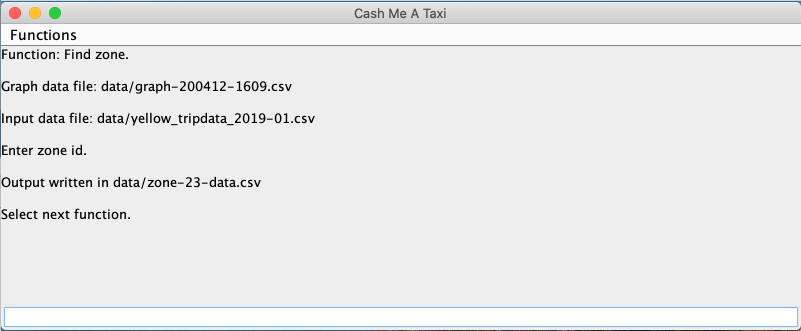
\includegraphics[scale = 0.7]{Images/FindZoneOutput.png}
    
    \item{You are now able to choose another function from the ``Functions" menu on the top menu bar.}
\ee

\subsubsection{Sort Edges}
\be
    \item{When ``Sort Edges" is chosen you will be given the following options. (Assuming you have already run the "Build Graph" function. If you have not, you will be prompted to input the file path. Return to \ref{BuildGraph} and repeat steps 2 and 3, before proceeding).}
    
        \item{You will now be prompted to choose how you would like the edges to be sorted. Enter the number, corresponding to the option you would like to choose, in the text box at the bottom of the window.}
    
    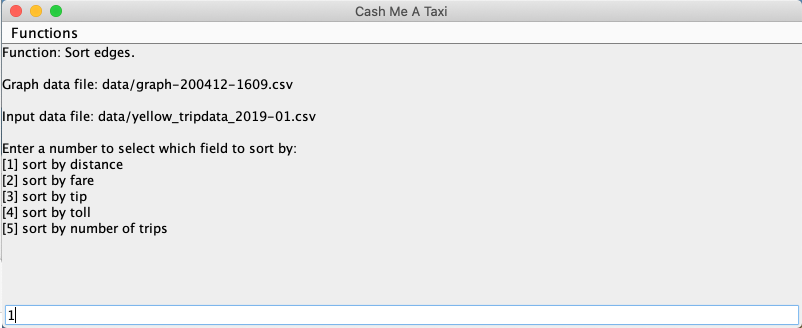
\includegraphics[scale = 1]{Images/SortEdgesData.png}
    
    \item{When you have chosen your option, the app sorts the data and stores them in the file specified.}
    
    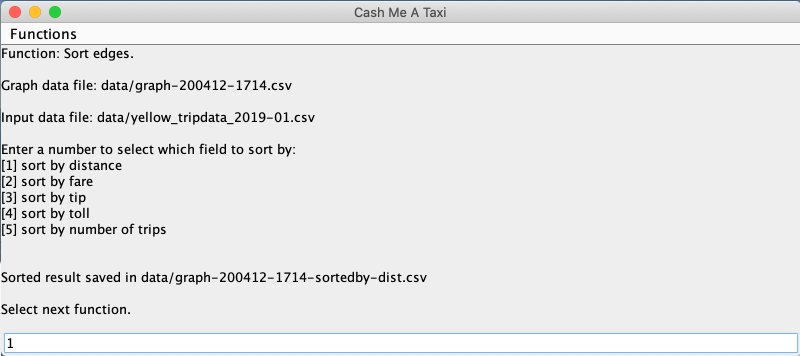
\includegraphics[scale = 1]{Images/SortEdgesOutput.png}
    
    \item{You are now able to choose another function from the ``Functions" menu on the top menu bar.}
\ee


\newpage

\section{Design Overview}

\subsection{Module Decomposition}

We wanted to emphasis the one module one secret idea so that many modules could be split up and implemented independently. We did not want the Graph module to be in charge of many tasks of the project, so we split them up into modules that use the Graph. The Parser is the only module that interacts with the input dataset to creates Trip objects that encapsulates the data of each dataset row. The Graph takes the Trips and creates Edges and Nodes to represent the graph. The SortedListOfEdges, GraphFind, and GraphSearch each contain the sorting, searching, and shortest path algorithms respectively. The GUI communicates with the user. The Controller takes the commands from the GUI, calls the appropriate tasks, then provides the GUI with the requested information.

\newpage

\subsection{UML Diagram}
Note that the relationships between modules are shown in the Uses diagram as there wasn't enough space to show all the uses relationships here.

\begin{center}
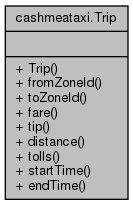
\includegraphics[scale = 0.6]{uml/classcashmeataxi_1_1Trip__coll__graph.png}
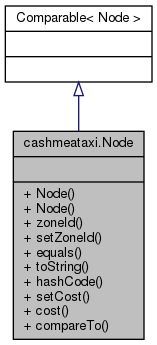
\includegraphics[scale = 0.6]{uml/classcashmeataxi_1_1Node__coll__graph.png} 
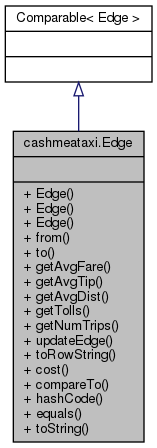
\includegraphics[scale = 0.6]{uml/classcashmeataxi_1_1Edge__coll__graph.png} 
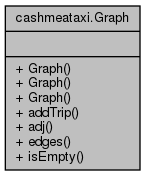
\includegraphics[scale = 0.6]{uml/classcashmeataxi_1_1Graph__coll__graph.png} 

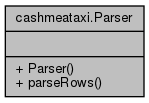
\includegraphics[scale = 0.6]{uml/classcashmeataxi_1_1Parser__coll__graph.png}
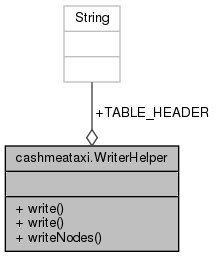
\includegraphics[scale = 0.6]{uml/classcashmeataxi_1_1WriterHelper__coll__graph.png}
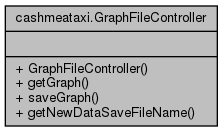
\includegraphics[scale = 0.6]{uml/classcashmeataxi_1_1GraphFileController__coll__graph.png} 

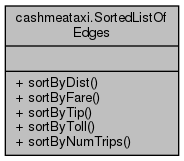
\includegraphics[scale = 0.6]{uml/classcashmeataxi_1_1SortedListOfEdges__coll__graph.png}
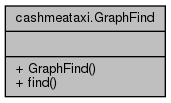
\includegraphics[scale = 0.6]{uml/classcashmeataxi_1_1GraphFind__coll__graph.png} 
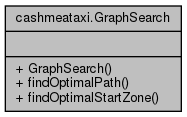
\includegraphics[scale = 0.6]{uml/classcashmeataxi_1_1GraphSearch__coll__graph.png} 

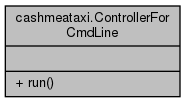
\includegraphics[scale = 0.6]{uml/classcashmeataxi_1_1ControllerForCmdLine__coll__graph.png} 
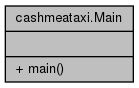
\includegraphics[scale = 0.6]{uml/classcashmeataxi_1_1Main__coll__graph.png} 

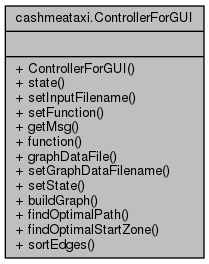
\includegraphics[scale = 0.6]{uml/classcashmeataxi_1_1ControllerForGUI__coll__graph.png} 
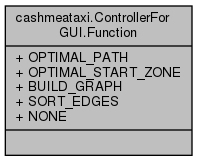
\includegraphics[scale = 0.6]{uml/enumcashmeataxi_1_1ControllerForGUI_1_1Function__coll__graph.png}
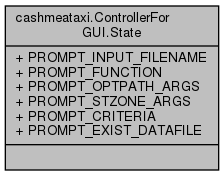
\includegraphics[scale = 0.6]{uml/enumcashmeataxi_1_1ControllerForGUI_1_1State__coll__graph.png}
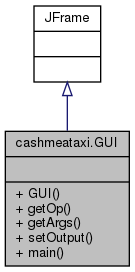
\includegraphics[scale = 0.6]{uml/classcashmeataxi_1_1GUI__coll__graph.png} 
\end{center}

\newpage

\subsection{Uses Relationship Diagram}

\begin{center}
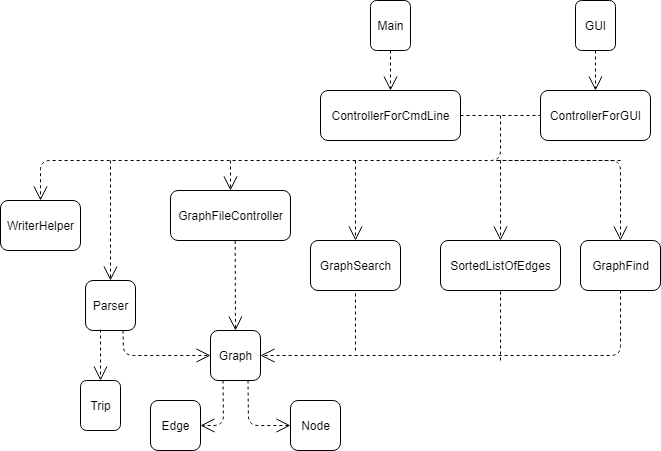
\includegraphics[scale = 0.70]{Images/Uses.png} 
\end{center}

\newpage

\section{Modules}

\subsection{Parser}

Parses the input dataset values into Trip data and then a Graph. 

The parser has no state variables and one function. Its purpose is to read the dataset and create a set of \code{Trip} objects representing the data of every row.

\subsubsection{Interface}

\bi
	\item \code{Parser(String inputDataFile)}
	\bi
		\item Create a new Parser given the filename for the dataset.
	\ei
	\item \code{long parseRows(Graph graph, long startRow, long numRowsToRead)}
	\bi
	    \item Ignore the first row (header) + \code{startRow} rows of the file.
		\item Reads rows up to \code{numRowsToRead}. For every row, parses the data, creates a \code{Trip} object, and adds it to \code{graph}.
		\item Returns the number of rows read.
	\ei
\ei

\subsubsection{Implementation Details}

Private entities:
\bi
	\item \code{final String inputFilename} The filename for the input dataset.
\ei

\noindent Notes:
\bi
	\item Uses a \code{BufferedReader} to read from the file.
	\item The reason why we want to specify the \code{startRow} when parsing data from the dataset is because if the dataset is very large and we've
	partially created a graph, we can continue from where we left off instead
	of starting all over again. 
\ei

\subsubsection{Requirements Traceback}

The parser meets the original requirements. It properly reads the file, but instead of creating a graph it grows it. 

\newpage

\subsection{Node}

A node represents a zone in New York City, with its id being the NYC taxi zone id. 

\subsubsection{Interface}
\bi
	\item \code{Node(int zoneId)}
	\bi
		\item Create a new Node given only the zone id.
	\ei
	\item \code{Node(int zoneId, String borough, int numStartTrips, int numEndTrips)}
	\bi
		\item Create a new Node.
	\ei
	\item \code{int zoneId()}
	\bi
		\item Get zone ID.
	\ei
	\item \code{void setZoneId(int zoneId)}
	\bi
		\item Set zone ID.
	\ei
	\item \code{boolean equals(Object other)}
	\bi
		\item Compare with another object.
		\item Returns \code{true} if the other object is a Node instance and its
		\code{zoneId} is the same is this object's \code{zoneId}.
	\ei
	\item \code{String toString()}
	\bi
		\item Return the string representation.
	\ei
	\item \code{int hashCode()}
	\bi
		\item Return the hash code.
	\ei
	\item \code{void setCost(Double cost)}
	\bi
		\item Set the cost. 
		\item Used for the graph search algorithm.
	\ei
	\item \code{Double cost()}
	\bi
		\item Get the cost.
		\item Used for the graph search algorithm.
	\ei
	\item \code{int compareTo(Node other)}
	\bi
		\item Compare with another \code{Node}.
		\item This object is greater than the given object if its cost is greater than the given Node's cost. 
	\ei
\ei

\subsubsection{Implementation Details}

Private entities:
\bi
	\item \code{int zoneId}
	\item \code{double cost} // for use in the graph search alg
\ei

\noindent Notes:
\bi
    \item \code{cost} is initially positive infinity. This is used for the graph search algorithm.
\ei

\subsubsection{Requirements Traceback}

The node meets the original requirements. It properly contains the contents of a New York City zone.

\newpage

\subsection{Edge}

An edge represents a connection from one \code{Node} to another. Its state variables include ID, starting \code{Node}, ending \code{Node}, average fare, average tips, average distance, tolls, trip count, and weight. It has a function \code{update} that updates its state when given a new \code{Trip}.

\subsubsection{Interface}

\bi
	\item \code{Edge(Node nodeFrom, Node nodeTo, long numTrips, double fare, double tip, double dist, double tolls)}
	\bi
		\item Create an Edge with the given data.
	\ei
	\item \code{Edge(Node nodeFrom, Node nodeTo, double fare, 
			double tip, double dist, double tolls)}
	\bi
		\item Create an Edge with the given data.
		\item This constructor doesn't require the \code{numTrips} field - it initializes the \code{numTrips} state variable as 1.
	\ei
	\item \code{Edge(Trip t)}
	\bi
		\item Create a new Edge given a Trip object.
		\item This constructor calls the second constructor above using the data retrieved from the given Trip object.
	\ei
	\item \code{Node from()}
	\bi
		\item Get source Node.
	\ei
	\item \code{Node to()}
	\bi
		\item Get destination Node.
	\ei
	\item \code{double getAvgFare()}
	\bi
		\item Get average fare.
	\ei
	\item \code{double getAvgTip()}
	\bi
		\item Get average tips.
	\ei
	\item \code{double getAvgDist()}
	\bi
		\item Get average distance.
	\ei
	\item \code{double getTolls()}
	\bi
		\item Get tolls.
	\ei
	\item \code{long getNumTrips()}
	\bi
		\item Get the number of trips.
	\ei
	\item \code{void updateTrip(Trip t)}
	\bi
		\item Updates the state variables when given a new \code{Trip} object.
		\item Recalculates its average fare, average tip and average distance fields given the new Trip object data. 
	\ei
	\item \code{String toRowString()}
	\bi
		\item Return the string representation.
	\ei
	\item \code{double cost()}
	\bi
		\item Return the cost in distance / money earned.
		\item This is used for the graph search algorithm.
	\ei
	\item \code{int compareTo(Edge other)}
	\bi
		\item Compare with another \code{Edge}.
		\item This object is greater than the given object if this cost() is greater than other.cost()
	\ei
	\item \code{int hashCode()}
	\bi
		\item Return the hash code.
	\ei
	\item \code{boolean equals(Object other)}
	\bi
		\item Compare with another object.
		\item This object is considered equivalent to the given object if its source nodes and destination nodes are equal.
	\ei
	\item \code{String toString()}
	\bi
		\item Return the string representation.
	\ei
\ei

\subsubsection{Implementation Details}

Private entities:

\bi
    \item \code{Node nodeFrom} // Source Node
    \item \code{Node nodeTo} // Destination Node
	\item \code{double avgFare} // Average fare
	\item \code{double avgTip} // Average tips earned
	\item \code{double avgDist} // Average Distance
	\item \code{double tolls} // Tolls
	\item \code{int numTrips} // Number of trips along the edge
\ei

\noindent Notes:
\bi
    \item \code{updateTrip(Trip t)} assumes the given \code{Trip} has the same source and end Nodes.
    \item The hash code is the integer equivalent of \code{nodeFrom.zoneId()} concatenated with \code{nodeTo.zoneId()}.
\ei

\subsubsection{Requirements Traceback}

The edge meets the original requirements. It properly represents the connection between 2 zones and updates when given new data.

\newpage

\subsection{Trip}

Wrapper class to encapsulate a single Trip record, whose data is retrieved from a single row in the dataset. 

\subsubsection{Interface}

\bi
	\item \code{Trip(int fromZoneId, int toZoneId, double fare, 
			double tip, double distance, double tolls, String startTime, String endTime)}
	\bi
		\item Create a \code{Trip} with the given data.
	\ei
	\item \code{int fromZoneId()}
	\bi
		\item Get source zone ID
	\ei
	\item \code{int toZoneId()}
	\bi
		\item Get destination zone ID
	\ei
	\item \code{double fare()}
	\bi
		\item Get the trip fare
	\ei
	\item \code{double tip()}
	\bi
		\item Get the tips
	\ei
	\item \code{double distance()}
	\bi
		\item Get distance
	\ei
	\item \code{double tolls()}
	\bi
		\item Get tolls
	\ei
	\item \code{String startTime()}
	\bi
		\item Get the start time
	\ei
	\item \code{String endTime()}
	\bi
		\item Get the end time
	\ei
\ei

\subsubsection{Implementation Details}

Private entities:

\bi
    \item \code{int from} // Starting zone
    \item \code{int to} // Ending zone
    \item \code{double fare} // Fare
	\item \code{double tip} // Tip
	\item \code{double distance} // Distance
	\item \code{double tolls} // Tolls
	\item \code{String startTime} // Start time
	\item \code{String endTime} // End time
\ei

\subsubsection{Requirements Traceback}

The trip meets the original requirements. It properly contains the contents from a row of the file.

\newpage

\subsection{Graph}

A collection of nodes and edges. Represents the directed graph with nodes representing a NYC zone, and edges between zones representing that taxi trips were made between these zones. 

\subsubsection{Interface}

\bi
	\item \code{Graph(ArrayList<Node> nodes)}
	\bi
		\item Create a \code{Graph} from the given \code{Node} list.
	\ei
	\item \code{Graph(List<Edge> edges)}
	\bi
		\item Create a \code{Graph} from the given \code{Edge} list.
	\ei
	\item \code{Graph()}
	\bi
		\item Create an empty \code{Graph}.
	\ei
	\item \code{void addTrip(Trip t)}
	\bi
	    \item Add an \code{Trip}. Add or update an edge to the graph given the new \code{Trip} object. 
	\ei
	\item \code{Iterable<Edge> adj(Node node)}
	\bi
		\item Get the adjacency list of the given \code{Node}.
	\ei
	\item \code{ArrayList<Edge> edges()}
	\bi
		\item Get the list of all \code{Edge}.
	\ei
	\item \code{boolean isEmpty()}
	\bi
		\item Determine if the \code{Graph} is empty.
	\ei
\ei

\subsubsection{Implementation Details}

Private entities:

\bi
	\item \code{Map<Node, HashMap<Node, Edge>>} adj - Adjacency map.
\ei

\noindent Notes:

\bi
    \item \code{adj} is a map with keys representing each node in the graph, and the values are a hashmap of \code{Node, Edge} where the \code{Node} represents a node it is connected to. The reason why we chose to use a hashmap instead of a linked list for each node is so that retrieving the edge between a given pair of nodes would be O(1). Retrieving the edge between nodes is done quite frequently, so it is a good idea to use a hashmap for the adjacency list instead of a linked list, which would have resulted in an O(n) retrieval time for an edge. 
\ei

\subsubsection{Requirements Traceback}

The graph meets the original requirements. It properly contains a collection of edges. Instead of updating with an edge it updates with a trip. A particular edge between a given pair of nodes can be fetched in O(1) time. 
\newpage

\subsection{GraphFind}

Find a node in the graph and retrieve its edges.

\subsubsection{Interface}

\bi
	\item \code{GraphFind(List<Edge> edges)}
	\bi
		\item Create a \code{GraphFind} object from the given \code{Edge} list.
	\ei
	\item \code{ArrayList<Edge> find(Node node)}
	\bi
		\item Return the list of of outgoing edges from the given node.
	\ei
\ei

\subsubsection{Implementation Details}

Private entities:

\bi
	\item \code{Map<Node, HashSet<Edge>>} graphAdjList - Adjacency map.
\ei

\noindent Notes:

\bi
    \item Searches using hashing, which takes O(1) time. 
\ei

\subsubsection{Requirements Traceback}

The searcher doesn't meets the original requirements. It originally searched for an edge, but a single edge is not very useful so instead it searches for all the outgoing edges of a node.

\newpage

\subsection{SortedListOfEdges}

Sorts a list of edges by a given field such as average distance, average fare, tips, tolls, and the number of trips made between the nodes in that edge. 

\subsubsection{Interface}

\bi
	\item \code{static void sortByDist(ArrayList<Edge> edgeList)}
	\bi
		\item Sorts the list of edges by distance
	\ei
	\item \code{static void sortByFare(ArrayList<Edge> edgeList)}
	\bi
		\item Sorts the list of edges by fare
	\ei
	\item \code{static void sortByTip(ArrayList<Edge> edgeList)}
	\bi
		\item Sorts the list of edges by tip
	\ei
	\item \code{static void sortByToll(ArrayList<Edge> edgeList)}
	\bi
		\item Sorts the list of edges by toll
	\ei
	\item \code{static void sortByNumTrips(ArrayList<Edge> edgeList)}
	\bi
		\item Sorts the list of edges by number of trips
	\ei
\ei

\subsubsection{Implementation Details}

\bi
    \item Sorts using a private class \code{Mergesort} that creates an \code{Edge[]} copy, sorts using standard merge sort with comparisons depending on the desired value, and copies the sorted array to the original. 
\ei

\subsubsection{Requirements Traceback}

The sorter meets the original requirements. It properly sorts a list of edges.

\newpage

\subsection{GraphSearch}

Traverses through the graph to search for the most optimal route between the given source node to the given destination node. 

\subsubsection{Interface}

\bi
	\item \code{GraphSearch(List<Edge> edges)}
	\bi
		\item Create a new \code{GraphSearch} object from the given \code{Edge} list.
	\ei
	\item \code{LinkedList<Node> findOptimalPath(int s, int e)}
	\bi
		\item Returns the most optimal path from the node specified by the zone id \code{s} to the node specified by the zone id \code{e}.
		\item The resulting linked list includes the start node (if the given start node exists in the graph), and then the nodes to the destination node that specify the most optimal route. If no optimal route is found, then only the start node is returned. 
	\ei
\ei

\subsubsection{Implementation Details}

Private entities:
\bi
	\item \code{Map<Node, HashSet<Edge>> adj} // Adjacency map that represents the graph.
\ei

\noindent Notes:

\bi
    \item \code{findOptimalPath} employs Dijkstra's Algorithm:
    \be
    	\item First find the start and end nodes in the graph that are specified by the given integer values that indicate the nodes' zone IDs. 
    	\item If either the start or end node don't exist, return an empty linked list. 
    	\item Set the ``cost" value of the start node to 0 (as per Dijkstra's algorithm).
    	\item Initialize a hashmap called \code{immediateParents<Node, Edge>} that will be used to track the immediate parents of each node to get the most optimal path.
    	\item Set all immediate parents to \code{null} (the keys in immediate parents are all the nodes in the graph).
    	\item Create a priority queue. Add the start node to the priority queue (as per Dijkstra's algorithm).
    	\item Enter a \code{while} loop. Remove the minimum cost node from the priority queue. If this minimum cost node has already been visited (we keep track of visited nodes in the set \code{visitedNodes}), then we \code{continue} in the while loop. 
    	\item Add the minimum cost node to the set of \code{visitedNodes}. Now visit this node's outgoing edges. For each outgoing edge whose destination node we have not visited yet, calculate a new cost (as per Dijkstra's algorithm) to this destination node, and if this new cost is less than its current cost, then set this node's cost to the new cost, and put the current outgoing edge as this node's immediate parent. 
    	Add the destination node of the outgoing edge to the priority queue to process later. 
    	\item Once we exit the while loop (when the priority queue is empty), we have found the most optimal (``shortest") path. This path data is stored in the \code{immediateParents} hashmap. We now start with the destination node, and add its immediate parent to an array list. Then we add the parent's node's immediate parent to the array list, and so forth until we reach the start node. 
    	\item The last thing to do is to reverse the array list and return it as a linked list which now has the correct optimal path from the source node to the destination node. 
    \ee
    \item To support the priority queue used in Dijkstra's algorithm described above, we modified our \code{Node} class to implement \code{Comparable<Node>} and have a function \code{compareTo(Node other)} that returns whether this node is of higher cost, lower cost or equal cost to the given node \code{other}. Because of this modification of the \code{Node} class, we can now easily use a \code{PriorityQueue} to hold a min heap of the nodes so that the retrieval of the minimum cost node is O(1) after every pass in the Dijkstra's algorithm. 
\ei

\subsubsection{Requirements Traceback}

The graph searcher was originally part of the controller. However we found that it is best to separate the graph search module from the controller to maintain separation of concerns. This module successfully finds the optimal path between the given two nodes.

\newpage

\subsection{WriterHelper}

Class to help write data onto csv files, specifically a list of edges or nodes from a graph.

\subsubsection{Interface}

\bi
   	\item \code{void write(String filename, List<Edge> edges)}
	\bi
		\item Write the list of \code{Edge} objects to a file, in csv format, with information of each edge such as the source/destination nodes, number of trips, average fare, average tips, etc.
	\ei
   	\item \code{void write(String filename, String pre, List<Edge> edges)}
	\bi
		\item Similar to above, but also writes a message before the table and then writes the csv-formatted table. 
	\ei
   	\item \code{void writeNodes(String filename, List<Node> nodes)}
	\bi
		\item Write the list of \code{Node} objects to a file, including each node's zone id. Writes each node on a separate line.
	\ei
\ei

\subsubsection{Implementation Details}

Private entities:
\bi
    \item \code{final static String TABLE\_HEADER} // The table header for the edges table.
\ei

\noindent Notes:
\bi
	\item Uses a \code{BufferedReader} to read from the file.
	\item Uses a \code{BufferedWriter} to write to the file.
\ei

\subsubsection{Requirements Traceback}

The writer helper wasn't originally part of the design. It was made to make file writing easier, which was also not part of the original design.

\newpage

\subsection{GraphFileController}

Manages the file IO to save graph data and read graph data from the graph data file. This module is used to save a graph onto a file so that we don't have to go through the process of building a new graph with the same input dataset; instead we could simply "load" an existing graph if we want to run some more functions. 

\subsubsection{Interface}

\bi
   	\item \code{GraphFileController(String dataFileName)}
	\bi
		\item Create a \code{GraphFileController} with the given filename.
	\ei
   	\item \code{Graph getGraph()}
	\bi
		\item Creates a new \code{Graph} object given the data on the graph data file. If there's no existing data, then return a new empty \code{Graph} object. 
		\item Assumes that this data file is valid. A valid graph data file must have the first line be ``numRowsReadFromInput=$<$number of rows read from the input data file$>$", the second line being the table header: \\``fromNode,toNode,numTrips,avgFare,avgTip,avgDistance,tolls", and each following line containing the above fields for each edge in the graph. 
	\ei
   	\item \code{void saveGraph(Graph graph, long deltaNumRowsRead)}
	\bi
		\item Save the given graph in the file determined by the state variable \code{filename} (which was initialized at the constructor). 
	\ei
   	\item \code{String getNewDataSaveFileName()}
	\bi
		\item Generate a new data file name, based on the current timestamp to avoid rewriting to existing graph data files. 
	\ei
\ei

\subsubsection{Implementation Details}

Private entities:
\bi
    \item String filename - Graph file name
\ei

\noindent Private functions:
\bi
	\item \code{void setupFile()}
	\bi
		\item Sets up the graph data output file. If the file given by the state variable \code{filename} already exists, then verify its contents to make sure its in the correct format.
		\item If the file given by the state variable \code{filename} does not exist or has invalid contents, then create a new file (overriding the existing one) and write the skeleton contents (i.e. the table header). 
	\ei
	\item \code{long getNumRowsRead()}
	\bi
		\item Get the number of rows that have been read from the input dataset. This number is saved in the first line of the graph data file specified by the state variable \code{filename}. 
	\ei
	\item \code{static void writeInitialContents(Writer fwriter)}
	\bi
		\item Given the file writer \code{fwriter}, write the initial skeleton contents for the graph data file (i.e. the table header and the number of lines read from input dataset value to 0). 
	\ei
	\item \code{static boolean verifyFile(File file)}
	\bi
		\item Verify the given file by making sure its contents meet the required format for the graph data file. 
	\ei
\ei

\noindent Notes:

\bi
	\item Uses a \code{BufferedReader} to read from the file.
	\item Uses a \code{BufferedWriterer} to write to the file.
\ei

\subsubsection{Requirements Traceback}

The graph file controller wasn't originally part of the design. It was created to save graph data so that we wouldn't have to repeatedly re-build the same graph based on the same input datasets. 

\newpage

\subsection{ControllerForCmdLine}

Controller for the command-line application. 

\subsubsection{Interface}
\label{sec:cmdlineinterface}

\bi
   	\item \code{void run(String[] args)}
	\bi
		\item Perform the appropriate functions based on the arguments.
		\item Command-line arguments: csvFilename functionToRun args loadExistingDataFile
	  	\bi
	  		\item functionToRun (required):
	  		\be
	  			\item Find optimal paths from zone A to zone B. Args required: startZone endZone
	  			\item Find zone. Args required: zone id
	  			\item Sort edges based on given a critera. Args required: criteriaId. criteriaId can be:
		  			\bi
		  				\item 1 - Sort by distance
		  				\item 2 - Sort by fare
		  				\item 3 - Sort by tip
		  				\item 4 - Sort by toll
		  				\item 5 - Sort by number of trips
		  			\ei
		  		\item Build graph. Required args: none
	  		\ee
	  		\item loadExistingDataFile (optional): load existing graph data that was previously saved by this program. Eg. raphdata-200309-1619.csv 
	  	\ei
	\ei
\ei

\subsubsection{Implementation Details}

Private entities:
\bi
    \item \code{String inputDataFile} // Input data
    \item \code{String saveDataFile} // Save data
	\item \code{Graph graph} // The graph
\ei

\noindent Private functions:
\bi
   	\item \code{void buildGraph(boolean readInputData)}
	\bi
		\item Build a graph and save the graph data into a file. This also sets the state variable \code{graph} with the \code{Graph} object created. 
		\item If \code{readInputData} is \code{true}, then read the input dataset specified by the state variable \code{inputDataFile} to build the graph.
		\item If \code{readInputData} is \code{false}, then build the graph based on an existing graph data file specified by the state variable \code{saveDataFile}. 
	\ei
   	\item \code{void findOptimalPath(String startZone, String endZone)}
	\bi
		\item Find the optimal path from one zone to another. Writes the result into a file.
	\ei
   	\item \code{void findZone(int zoneId)}
	\bi
		\item Find a zone given by the zone ID. Writes the result into a text file. 
	\ei
   	\item \code{void sortEdges(int criteria)}
	\bi
		\item Sort the \code{graph} edges based on a criteria.
	\ei
   	\item \code{void buildGraph()}
	\bi
		\item Builds the graph. 
		\item First checks if there is an existing graph data file specified by a non-empty \code{saveDataFile}. If there is, then build the graph without reading the input dataset. If there is no existing graph data file specified, then builds the graph by reading the input dataset. 
	\ei
\ei
\subsubsection{Requirements Traceback}

The controller meets most of the original requirements. It properly makes the graph on startup and performs the functions. It doesn't update the graph as the graph doesn't change, or use the GUI as the GUI is the higher entity.

\newpage

\subsection{Main}

Main class for the command-line application.

\subsubsection{Interface}

\bi
   	\item \code{static void main(String[] args)}
	\bi
		\item Run the \code{ControllerForCmdLine}.
		\item The \code{args} passed to \code{main} must follow the rules specified in the \code{ControllerForCmdLine} specifications. 
	\ei

\ei

\newpage

\subsection{ControllerForGUI}

Controller for the GUI application.

\subsubsection{Interface}

\bi
	\item \code{ControllerForGUI()}
	\bi
	    \item Create a new \code{ControllerForGUI} object.
	    \item Initialize the state variable \code{state} to \code{State.PROMPT\_FUNCTION}. 
	    \item Initialize the state variable \code{function} to \code{Function.NONE}.
	\ei
	\item \code{enum State}
	\bi
		\item Current state of the GUI application. 
		\item Values:
		\bi
			\item \code{PROMPT\_INPUT\_FILENAME}
			\item \code{PROMPT\_FUNCTION}
			\item \code{PROMPT\_OPTPATH\_ARGS}
			\item \code{PROMPT\_FZONE\_ARGS}
			\item \code{PROMPT\_CRITERIA}
			\item \code{PROMPT\_EXIST\_DATAFILE}
		\ei
	\ei
	\item \code{enum Function}
	\bi
		\item Current function that is to be run by the user. 
		\item Values:
		\bi
			\item \code{OPTIMAL\_PATH}
			\item \code{FIND\_ZONE}
			\item \code{BUILD\_GRAPH}
			\item \code{SORT\_EDGES}
			\item \code{NONE}
		\ei
	\ei
	\item \code{State state()}
	\bi
		\item Return the current state.
	\ei
	\item \code{void setInputFilename(String filename)}
	\bi
		\item Set the input dataset filename.
	\ei
	\item \code{void setFunction(Function f)}
	\bi
		\item Set the function to run.
	\ei
	\item \code{String getMsg()}
	\bi
		\item Return the message to display on the GUI depending on the current state and function being run.
	\ei
	\item \code{Function function()}
	\bi
		\item Return the current function that is to be run.
	\ei
	\item \code{String graphDataFile()}
	\bi
		\item Return graph data file. 
	\ei
	\item \code{void setGraphDataFilename(String filename)}
	\bi
		\item Set the save filename to save the graph data.
	\ei
	\item \code{void setState(State state)}
	\bi
		\item Set the current state.
	\ei
	\item \code{String buildGraph(boolean readInputData)}
	\bi
		\item Build \code{graph} and return the filename that the graph data is stored in.
		\item If \code{readInputData} is \code{false}, then that means we don't want to read the input dataset, and we can build the graph from an existing graph data file. 
		\item If \code{readInputData} is \code{true}, then we must read the input dataset and build the graph based off of that. 
	\ei
   	\item \code{String findOptimalPath(int startZone, int endZone)}
	\bi
		\item Find the optimal path given the start and end zone IDs.
		\item Writes the resulting output to a file, and returns the filename of where the output is saved. 
	\ei
   	\item \code{String findZone(int zoneId)}
	\bi
		\item Find the zone given by its id.
		\item Writes data on the zone's outgoing edges in a file. Returns the name of this file.
	\ei
   	\item \code{String sortEdges(int criteria)}
	\bi
		\item Sort the graph's edges by a field specified by the \code{criteria}. 
		\item Sorted in ascending order. 
		\item Writes the sorted edges output on a file. Returns the name of this file.
	\ei
\ei

\subsubsection{Implementation Details}

Private entities:
\bi
	\item \code{String inputDataFile} // Input dataset file
	\item \code{String saveDataFile} // Graph data file to save the graph
	\item \code{Graph graph} // Graph
	\item \code{State state} // Current state of the GUI application
	\item \code{Function function} // The current function that is to be run
\ei

\noindent Private functions:
\bi
   	\item \code{void buildGraph()}
	\bi
		\item Builds the graph. 
		\item First checks if there is an existing graph data file specified by a non-empty \code{saveDataFile}. If there is, then build the graph without reading the input dataset. If there is no existing graph data file specified, then builds the graph by reading the input dataset. 
	\ei
\ei

\subsubsection{Requirements Traceback}

The controller meets most of the original requirements. It properly makes the graph on startup and performs the functions. It doesn't update the graph as the graph doesn't change, or use the GUI as the GUI is the higher entity.

\subsubsection{UML State Machine}

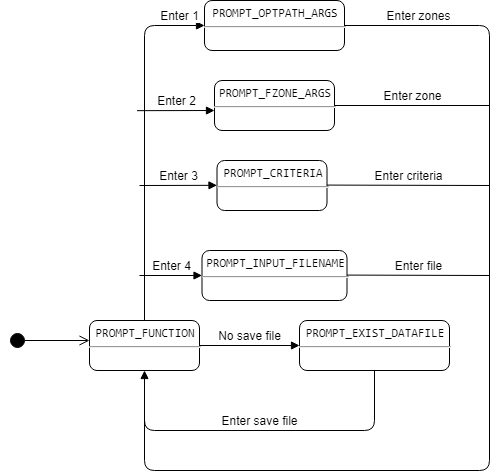
\includegraphics[scale = 0.75]{Images/ControllerForGUIDiagram.png} 

\newpage

\subsection{GUI}

Main class for the GUI application. Extends the Java \code{JFrame} module. 

\subsubsection{Interface}

\bi
	\item \code{GUI()}
	\bi
	    \item Create the GUI with a menu bar at the top, the input text at the bottom, and the output label between them.
		\item When a menu option is selected, set the appropriate option and display the prompt.
		\item Run the appropriate function and save the results to a file.
	\ei
    \item \code{static void main(String[] args)}
    \bi
        \item The main function to run when running the GUI application.
    \ei
\ei

\subsubsection{Implementation Details}

Private entities:
\bi
	\item \code{JTextField input} // Input textbox
	\item \code{JLabel output} // Output label
	\item \code{JMenuBar menu} // Menu bar
	\item \code{ControllerForGUI controller} // Controller
\ei

\noindent Private functions:
\bi
	\item \code{static void setOutput(String text)}
	\bi
		\item Set the text of \code{output} line by line. 
	\ei
    \item \code{static void validateZone(int zone)}
    \bi
        \item Validates the zone ID inputted by the user. The zone must be between 1 and 263, which is the range of valid NYC taxi zones.
        \item Throws a new IllegalArgumentException if the zone is not valid. The calling function then catches the exception and displays an error message on the GUI, and prompts the user to select a new function.
    \ei
    \item \code{static void validateSortOption(int option)}
    \bi
        \item Validates the sorting criteria option inputted by the user. The option must be between 1 and 5. 
        \item Throws a new IllegalArgumentException if the option is not valid. The calling function then catches the exception and displays an error message on the GUI, and prompts the user to select a new function.
    \ei
\ei

\noindent Notes:

\bi
    \item The GUI is implemented using Java Swing.
    \item It is a frame containing a menu, input textbox, and output label.
    \item When a menu option is selected the corresponding function is called via \code{controller}. If arguments are needed the user is given a prompt first.
    \item The function's output is displayed on \code{output} line by line.
\ei

\subsubsection{Requirements Traceback}

The GUI meets most of the original requirements. It properly makes accepts user input. Since most of the output will be too large to display, it is instead written to a file.

\subsubsection{UML State Machine}

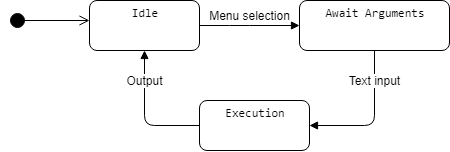
\includegraphics[scale = 0.80]{Images/GUIDiagram.png}

\newpage

\section{Design Critique}

The non-functional requirements set out by the SRD have been met. The application is always available as it only relies on files on the computer. It is secure as there is no personal data required. It is completely safe to use. Since the dataset is static, it is up to the user to update it to ensure the results are accurate. The performance is relatively fast compared to the size of the data. The memory usage is large as the dataset is large. The user interface could have some improvements such as shortcuts so that entire file paths don't have to be typed or a legend to map zones with real-world locations. The program is still constrained by the presence of the large dataset, but it can be used for other city datasets as long as they meet the same format. Running only on a computer with Java correctly installed is still a big constraint, but it shouldn't be a problem as it is not heavily used by the small audience.

Although the graph ``saving" parts aren't completely necessary as the graph can be re-built everytime, we believe that as the dataset grows, it become significantly faster to run multiple functions over multiple runs of the program using the same dataset, since the graph will only be built once and subsequent program runs can use the already-constructed graph data to perform computations. 

\end{document}
